% paper proposal for the Modelica 2017 Conference

%%% By default the modelica LaTeX class uses bibtex and natbib for refrences
\documentclass{resources/modelica}
%%% As alternative also for unicode and @online support
%%% use the more modern biber and biblatex instead
%\documentclass[backend=biber]{modelica}
%\addbibresource{example-paper.bib}
%\usepackage[utf8]{luainputenc} % utf8 input encoding that should work for both pdflatex and lualatex, but might not be available in every installation
\usepackage[utf8]{inputenc} % utf8 input encoding which should work with pdflatex, but not lualatex
\usepackage{cleveref}
%\usepackage{xcolor}
\usepackage{caption} % subfloats (http://en.wikibooks.org/wiki/LaTeX/Floats,_Figures_and_Captions#Subfloats)
\usepackage{subcaption} % subfloats (http://en.wikibooks.org/wiki/LaTeX/Floats,_Figures_and_Captions#Subfloats)
\usepackage{lmodern}
\usepackage{textcomp}

\hypersetup{%
  pdftitle  = {Towards a Standard-Conform, Platform-Generic and Feature-Rich Modelica Device Drivers Library},
  pdfauthor = {Bernhard Thiele, Thomas Beutlich, Volker Waurich, Martin Sjölund,
  Tobias Bellmann}, pdfsubject = {12th International Modelica Conference 2017},
  pdfkeywords = {Modelica, embedded systems, real-time simulation},
  colorlinks,
  linkcolor=black,
  urlcolor=black,
  citecolor=black,
  pdfpagelayout = SinglePage,
  pdfcreator = pdflatex,
  pdfproducer = pdflatex}

\lstset{language = c,
       % basicstyle=\fontsize{9pt}{10.5pt}\selectfont,
       basicstyle=\fontsize{9pt}{10.5pt}\ttfamily,
       backgroundcolor = \color{white}}

\newcommand{\clang}[1]{\lstinline[language=c]|#1|}
\newcommand{\modelica}[1]{\lstinline[language=modelica]|#1|}

% \newcommand{\BTHI}[1]{{\color{blue}{$\parallel_\textrm{BTHI}$#1$\parallel$}}}
% \newcommand{\TBEU}[1]{{\color{orange}{$\parallel_\textrm{TBEU}$#1$\parallel$}}}
% \newcommand{\VWAU}[1]{{\color{red}{$\parallel_\textrm{VWAU}$#1$\parallel$}}}
% \newcommand{\MSJO}[1]{{\color{green}{$\parallel_\textrm{MSJO}$#1$\parallel$}}}
% \newcommand{\TBEL}[1]{{\color{magenta}{$\parallel_\textrm{TBEL}$#1$\parallel$}}}
\newcommand{\BTHI}[1]{}
\newcommand{\TBEU}[1]{}
\newcommand{\VWAU}[1]{}
\newcommand{\MSJO}[1]{}
\newcommand{\TBEL}[1]{}


\crefformat{footnote}{#2\footnotemark[#1]#3}

% begin the document
\begin{document}
\thispagestyle{empty}

\title{Towards a Standard-Conform, Platform-Generic and Feature-Rich Modelica Device Drivers Library}
\author[1]{Bernhard Thiele}
\author[2]{Thomas Beutlich}
\author[3]{Volker Waurich}
\author[1]{Martin Sjölund}
\author[4]{Tobias Bellmann}
\affil[1]{PELAB, Linköping University, Sweden, {\small\texttt{\{bernhard.thiele,martin.sjolund\}@liu.se}}}
\affil[2]{ESI ITI GmbH, Germany, {\small\texttt{thomas.beutlich@esi-group.com}}}
\affil[3]{Chair of Construction Machinery, TU Dresden, Germany, {\small\texttt{volker.waurich@tu-dresden.de}}}
\affil[4]{Institute of System Dynamics and Control, DLR, Germany, {\small\texttt{tobias.bellmann@dlr.de}}}

\date{} % <--- leave date empty
\maketitle\thispagestyle{empty} %% <-- you need this for the first page
\abstract{%
There are many cases where simulation applications need to interact with their
environment. Typical examples are Human-in-the-Loop (HITL) simulators (including
flight, driving, and marine training simulators), Hardware-in-the-Loop (HIL)
simulators, but also offline process simulators which cannot operate in a
completely self-contained manner and therefore need to be coupled to external
applications. Embedded control applications are another related area
requiring interaction between applications and their environment. The
\emph{Modelica\_DeviceDrivers} library, which had its first release as
open-source library in 2012, tries to cater to such use cases. This paper
describes the library for the first time and reports about the numerous
challenges that the project experienced to meet its goal of supporting several
platforms and tools within a standard-conform, platform-generic, feature-rich,
and easy-to-use Modelica library.
Furthermore, the paper gives an insight into the inner mechanics of the
library's communication and serialization functionalities, the various
supported hardware interfaces and the possibilities to generate code
for embedded systems.
}

\noindent\emph{Keywords: human-in-the-loop, hardware-in-the-loop, real-time simulation, embedded control application,
Modelica external C}

\section{Introduction}
\label{sec:Introduction}
\BTHI{Bernhard, Tobias}

The most common usage of Modelica models is for offline simulation experiments.
However, in many cases simulations need to interact with their environment or
other software components.
Typical examples are Human-in-the-Loop (HITL) simulators (including flight,
driving, and marine training simulators), Hardware-in-the-Loop (HIL) simulators,
but also offline process simulators which cannot operate in a completely
self-contained manner and therefore need to be coupled to external applications.
Furthermore, Modelica can be used for developing (model-based) control
applications which also require interaction with their environment.

There are different approaches for enabling the above mentioned applications in
the context of Modelica. Several simulator devlopment environments offer tool chains for
real-time simulation and/or model-based development of embedded control
applications. Modelica tools may interface these simulator devlopment environments, by wrapping the generated, third-party-specific code
from the Modelica tool into tool-internal representations, which then can be connected to hardware devices in the respective simulator devlopment environment. For example, such customized solutions are available in
\begin{itemize}
 \item Dymola\footnote{Dassault Systèmes, \url{https://www.3ds.com}} via its DymolaBlock interface to the MATLAB/Simulink\footnote{\label{tmw}The MathWorks, \url{https://mathworks.com}} tool chain
 \item OpenModelica\footnote{Open Source Modelica Consortium (OSMC), \url{https://www.openmodelica.org}} via customized tool chains \citep{Worschech2012}
 \item SimulationX\footnote{SimulationX by ESI, \url{https://www.simulationx.com}} via Code Export for Simulink/Simulink Coder\cref{tmw} or HIL environments like dSPACE DS1006\footnote{\label{dspace}dSPACE, \url{https://www.dspace.com}}, NI VeriStand\footnote{National Instruments, \url{http://www.ni.com}} or ETAS LAB\-CAR\footnote{ETAS, \url{http://www.etas.com}} \citep{Blochwitz2009}
\end{itemize}
Furthermore, it may also be possible for Modelica tools to generate Functional
Mock-up Units\footnote{FMI development group,
\url{https://www.fmi-standard.org}} (FMUs) which can be imported into compatible simulator
development environments (\textit{e.g.}, the tool chain provided for the dSPACE SCALEXIO\cref{dspace} platform).

Instead of embedding the (FMI-) compiled Modelica model into a simulator
environment, the \emph{Modelica\_DeviceDrivers} (MDD) library uses a different approach.
The MDD library provides access to external devices by utilizing Modelica's external
function interface for interfacing to the C API of various device drivers directly from Modelica
models (see Section~\ref{ModelicaDeviceDrivers}).

Historically, the origins of the MDD library can be traced back to the
\emph{ExternalDevices} library \citep{Bellmann2009}, an internal
DLR\footnote{Deutsches Zentrum für Luft- und Raumfahrt (DLR), German Aerospace
Center, \url{http://www.dlr.de}} Modelica library developed for the interactive
simulation and visualization of Modelica models. The \emph{ExternalDevices}
library already supported UDP and shared memory communication
as well as several input devices (keyboard, 3Dconnexion
SpaceMouse\footnote{3Dconnexion, \url{https://www.3dconnexion.com}}, and game
controller). Additionally, it featured a model-integrated real-time
visualization system, the foundation of the later \emph{DLR Visualization} library \citep{Hellerer2014}.

However, the \emph{ExternalDevices} library only supported
Microsoft Windows and was developed and tested using only the Dymola tool,
which caused unintentional incompatibilities with other Modelica tools.
In the further course of
development it was decided to split the \emph{ExternalDevices} library into the
commercial \emph{DLR Visualization} library and an open-source cross-platform hardware
interface library, the \emph{Modelica\_DeviceDrivers} library. The library is
available from its GitHub project site at
\url{https://github.com/modelica/Modelica_DeviceDrivers/}.
This paper is based on MDD v1.5.0, the latest release version.


% \BTHI{TODO: Bernhard, Tobias , \cite{Elmqvist2009}}


\section{Modelica\_DeviceDrivers}
\label{ModelicaDeviceDrivers}
\BTHI{TODO: Bernhard, Thomas, Volker}

The MDD library allows to access hardware devices from Modelica models.
This is achieved by using the Modelica external C interface to call the
appropriate C driver functions provided by the underlying operating system (see
Section~\ref{sec:CrossPlatformSupport}).

The library is organized in several layers as indicated in
Figure~\ref{fig:MDDLayeredArchitecture}. It
provides two high-level Drag \& Drop block interfaces. The first (\texttt{Blocks}) is
compatible to Modelica 3.2, using the traditional \modelica{when sample()}
element for periodically calling Modelica functions from the \textsf{Function Layer}. The second
(\texttt{ClockedBlocks}) uses the synchronous language elements extension
introduced in Modelica 3.3 and is compatible with the
\emph{Modelica\_Synchronous} library \citep{Otter2012}. Due to this support, the
MDD library formally depends on the \emph{Modelica\_Synchronous} library, but in
practice the \emph{Modelica\_Synchronous} library (and tool support for the
synchronous language elements extension) is only required if one actually wants
to use the clocked block interface.
\begin{figure}[htb]
\begin{center}
  \includegraphics[width=\columnwidth]{figures/MDDLayeredArchitecture}
  \caption{MDD layered architecture.}
  \label{fig:MDDLayeredArchitecture}
\end{center}
\end{figure}

\subsection{Cross-Platform Support}
\label{sec:CrossPlatformSupport}

As of MDD v1.5.0, Windows and Linux are supported as main platforms,
but prototypical work also targets popular embedded systems boards directly (see
Section~\ref{sec:EmbeddedControl}).

When accessing hardware devices, a Modelica model or
application calls Modelica functions from the \textsf{Function Layer} (see
Figure~\ref{fig:MDDLayeredArchitecture}). These Modelica functions provide a
generic interface to the underlying \textsf{C Code Layer} which is accessed by
Modelica's external function interface.
The platform differentiation is handled in the \textsf{C Code Layer} which
uses preprocessor directives for conditional inclusion/exclusion of
platform-specific code (\mbox{\clang{#if}}, \mbox{\clang{#else}},
\mbox{\clang{#endif}}, etc.) similarly to the code fragment below.
\begin{lstlisting}[language=C]
#if defined(_MSC_VER) || defined(__CYGWIN__) || defined(__MINGW32__)
#include <windows.h>
/* Windows specific code goes here */
#elif defined(__linux__)
#include <unistd.h>
/* Linux specific code goes here */
#else
#error "Modelica_DeviceDrivers: Unsupported compiler or platform"
#endif
\end{lstlisting}

\subsection{Extended Tool Support}
\label{sec:ExtendedToolSupport}

Back in 2009, the library was developed using the Dymola tool. With MDD v1.4.0,
considerable development efforts have been spent on the Modelica compliance of
the library in order to better support SimulationX and OpenModelica.

Since OpenModelica 1.11 Beta 1 the MDD Communication blocks are finally
supported by OpenModelica. For achieving this, it was necessary to change parts
of the library (under the constraint of maintaining backwards compatibility),
and at the same time, to extend the abilities of respective tools (partly by
providing support for constructs which are not (yet) allowed by the Modelica
language standard). This is discussed in more detail in
Section~\ref{sec:ModelicaStandardCompliance}.


\subsection{Library Structure}
\label{sec:LibraryStructure}

Figure~\ref{fig:MDDPackageBrowseScreenshot} shows a screenshot of the package
browser view with loaded MDD library. The first two sub-packages
\modelica{Blocks} and \modelica{ClockedBlocks} provide the drag \& drop blocks
which correspond to the \textsf{Block Layer} of
Figure~\ref{fig:MDDLayeredArchitecture}. The remaining sub-packages (except
\modelica{Utilities} and \modelica{EmbeddedTargets}) provide the
\textsf{Function Layer}.
Both layers use sub-packages for subdividing the provided functionality into
different groups. Package \modelica{EmbeddedTargets} contains highly
target specific function and blocks for supporting restricted
embedded systems like the Arduino microcontroller (see
Section~\ref{sec:Applications}).

\begin{figure}[htb]
  \centering
  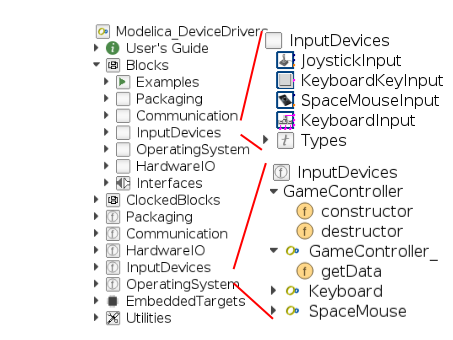
\includegraphics[width=\columnwidth]{figures/MDDPackageBrowseScreenshot}
  \caption{MDD library structure.}
  \label{fig:MDDPackageBrowseScreenshot}
\end{figure}

Furthermore, Figure~\ref{fig:MDDPackageBrowseScreenshot} gives an indication
about the relation between the \textsf{Block Layer} and the \textsf{Function Layer}. Typically, a
device driver block will instantiate a corresponding external object from the
\textsf{Function Layer}. Modelica's external objects allow to maintain internal memory
between calls to external functions. This allows to open and initialize hardware
devices once, during Modelica's initialization phase, and maintain the so
created device handlers in memory for accessing them in subsequent simulation phases.
For example, the \modelica{JoystickInput} block creates an instance of the
external object class \mbox{\modelica{GameController}.} The package
\modelica{GameController_} collects functions that can operate on external
objects of type \modelica{GameController}. The package provides the function
\modelica{getData}, which takes a \modelica{GameController} object as
argument and returns the values of the axes and buttons of its associated
hardware device.

A good way of learning how to use the \textsf{Block Layer} interface of the library is by
exploring the \modelica{Examples} package. Care has been taken to provide
self-explanatory usage examples for the provided device driver blocks.

\subsection{Interfaces}

MDD library functionality can be accessed by drag \& drop of blocks
from the \modelica{Blocks} and \modelica{ClockedBlocks} sub-packages, or by
direct calls to the underlying functions.

An example, which directly uses the \textsf{Function Layer} for accessing a
game controller is given below:
\begin{lstlisting}[language=modelica]
model GameControllerExample
  import
    Modelica_DeviceDrivers.InputDevices.*;
  parameter Integer id = 0 "0 = first attached game controller";
  GameController gc = GameController(id);
  discrete Real axesRaw[6];
  Integer buttons[32], pOV;
equation
  when sample(0,0.1) then
    (axesRaw,buttons,pOV) = GameController_.getData(gc);
  end when;
end GameControllerExample;
\end{lstlisting}

\noindent
The code above creates an external object named \mbox{\modelica{gc}.} The
constructor for this object takes the argument \mbox{\modelica{id}.} This
argument allows to specify which controller to use if several game controllers are attached to the
system. The function \modelica{getData} is called periodically within a
\modelica{when}-clause. It takes the external object \modelica{gc} as
argument and returns vectors which contain the values read from the
associated game controller. The vector is pre-dimensioned, so that it can attune
to controllers featuring as much as six axes, 32 buttons and a POV (point of
view) switch. The actually available data depends on the connected game
controller hardware. Tests with the actual hardware are needed for determining
which vector entry corresponds to which physical axis or button.

Figure~\ref{fig:JoystickBlocks} shows how game controllers can be accessed by
simply dragging \& dropping a \modelica{JoystickInput} block into the diagram
view of a Modelica tool. While Figure~\ref{fig:MDDJoystick} uses the block found
in the \modelica{Blocks} package,
Figure~\ref{fig:MDDJoystickClocked} uses the corresponding clocked variant from
\modelica{ClockedBlocks}. The additional blocks \modelica{periodicClock} and
\modelica{assignClock} are from the \emph{Modelica\_Synchronous} library. They
associate a periodic clock to the variables and equations within the
\modelica{JoystickInput} block. As a result, the underlying
\modelica{getData} function will be called whenever the
associated clock ticks (\textit{i.e.}, every $0.1\,\mathrm{s}$ in the presented
example).

\begin{figure}[htb]
  \centering
  \begin{subfigure}[b]{0.45\columnwidth}
     \centering
     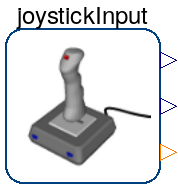
\includegraphics[width=0.55\textwidth]{figures/MDDJoystick}
     \caption{Using \modelica{Blocks}}
     \label{fig:MDDJoystick}
  \end{subfigure}%
  ~ %add desired spacing between images, e. g. ~, \quad, \qquad, \hfill etc.
    %(or a blank line to force the subfigure onto a new line)
  \begin{subfigure}[b]{0.45\columnwidth}
          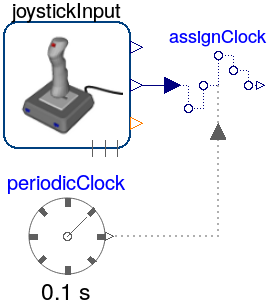
\includegraphics[width=\textwidth]{figures/MDDJoystickClocked}
          \caption{Using \modelica{ClockedBlocks}}
          \label{fig:MDDJoystickClocked}
  \end{subfigure}
  \caption{Accessing game controller devices by using the
  \modelica{JoystickInput} block from the \modelica{Blocks}, or the
  \modelica{ClockedBlocks} package.}
  \label{fig:JoystickBlocks}
\end{figure}

\noindent
The example models can be simulated, but real-time synchronization is
required to slow the simulation speed down, in order to synchronize the
real-time inputs with the simulation progress.
The MDD library provides convenient support for (soft) real-time
synchronization\footnote{See documentation to block
\mbox{\modelica{SynchronizeRealtime}.}
%\url{https://build.openmodelica.org/Documentation/Modelica_DeviceDrivers.Blocks.OperatingSystem.SynchronizeRealtime.html}
}.
However, a user should consider that Modelica tools may provide better (tool-specific) mechanisms for real-time synchronization.

\subsection{Features}

The MDD library has grown to support a respectable amount of hardware devices
and associated features which will be briefly presented in this section.

\subsubsection{Input Devices}
\begin{figure}[htb]
  \centering
  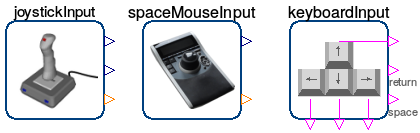
\includegraphics[width=0.7\columnwidth]{figures/OverviewInputDevices}
  \caption{Supported input devices from the \modelica{Blocks} package.}
  \label{fig:OverviewInputDevices}
\end{figure}

\noindent
Standard input devices such as keyboard and game controllers are ubiquitously
available on the market, enabling the user to quickly build up interactive simulations.
MDD provides blocks for using the generic keyboard and game controller interface
of Windows or Linux (see Figure~\ref{fig:OverviewInputDevices}). Also more
specialized hardware like the 3Dconnexion SpaceMouse is supported for both platforms.
Often, these blocks will be used for interactive desktop simulations, but they
can also become part of more involved (cost-efficient) HITL simulation
scenarios.

\subsubsection{Communication}
\label{sec:Communication}

The most comprehensive and complex part of the library is related to
communication devices and their supporting Modelica and external C code.

\paragraph{Supported Devices}

\begin{figure}[htb]
  \centering
  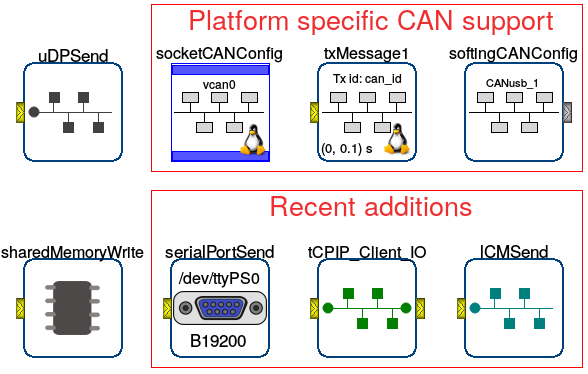
\includegraphics[width=0.9\columnwidth]{figures/OverviewCommunicationDevices}
  \caption{Supported communication devices from the \modelica{Blocks} package.}
  \label{fig:OverviewCommunicationDevices}
\end{figure}


Figure~\ref{fig:OverviewCommunicationDevices} gives an overview over the
supported devices. Cross-platform support for UDP and shared memory was already
available in the first released version of MDD. Support for serial port communication is
available since MDD v1.3 (Linux) and v1.4.0 (Windows). A client block for TCP/IP
socket communication was added in v1.4.0 (Windows) and v1.5.0 (Linux).
Furthermore, support for sending and receiving of Lightweight Communications and
Marshalling (LCM) datagrams\footnote{LCM project,
\url{https://lcm-proj.github.io}} was added in v1.5.0.
LCM is a set of libraries and tools for message passing and data marshalling,
which is particularly targeted at low-latency real-time applications for
robotic systems \citep{Huang2010}.

Basic support for the Controller Area Network bus (CAN bus) is available by two
different block sets. The first is based on the CAN Layer2 API from
Softing\footnote{Softing, \url{http://industrial.softing.com}} and restricted to the
Windows platform. The second uses the SocketCAN
interface provided by the Linux kernel.

\paragraph{Packaging Concept}

Communication devices like UDP or shared memory use a common packaging concept
in order to send or receive data. Therefore, the same packager can be used with
different communication devices. Figure~\ref{fig:PackagingConcept} shows an
example in which a package consisting of three variables of type \modelica{Real}
followed by a variable of type \modelica{Integer} is either transmitted using
shared memory or UDP blocks. Switching between the two communication devices
is achieved by simply replacing the corresponding device block.

\begin{figure}[htb]
  \centering
  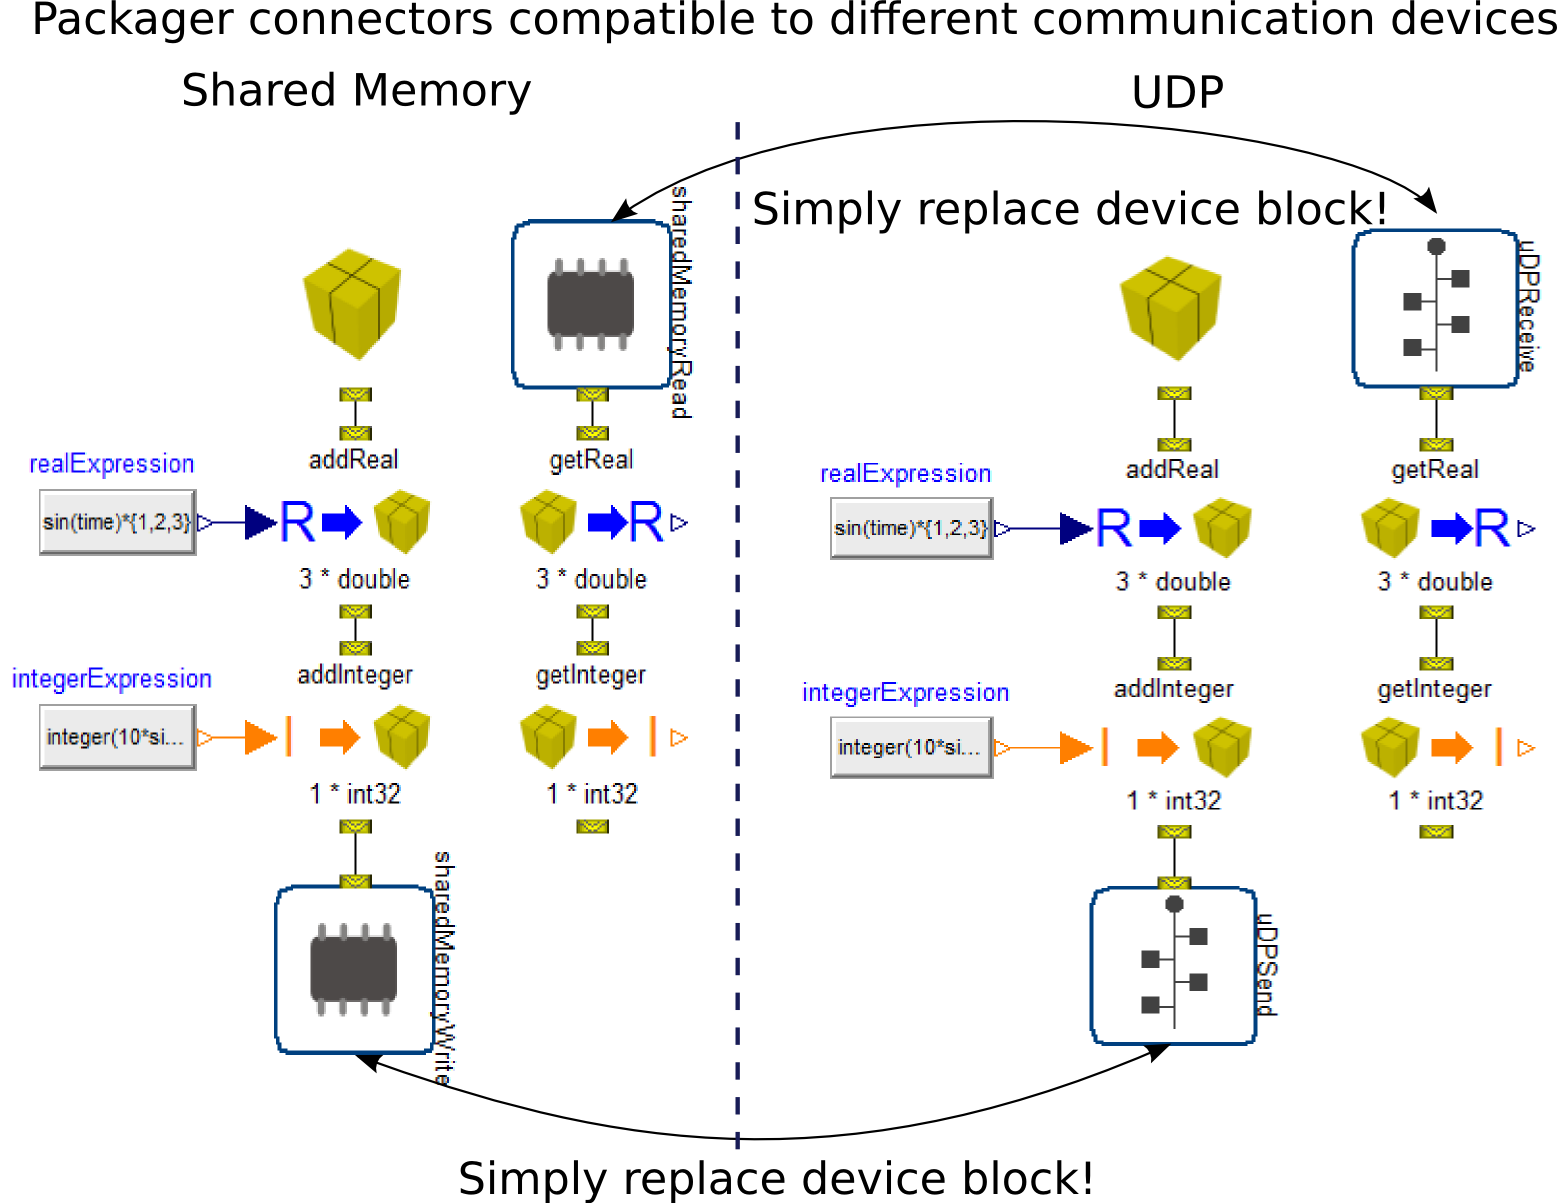
\includegraphics[width=1.0\columnwidth]{figures/PackagingConcept}
  \caption{Simple switching of communication devices due to common packaging concept
  in order to send or receive data.}
  \label{fig:PackagingConcept}
\end{figure}

\noindent
The packages are constructed by using blocks from the \modelica{Packaging}
sub-package (see Figure~\ref{fig:MDDPackageBrowseScreenshot}). In the initial
design of MDD it was expected that different packaging concepts would be
supported which share a common connector interface. However, as of MDD v1.5.0
the \modelica{SerialPackager} is the only available packager. It allows
to periodically add (or retrieve) fixed size vectors to (or from) a package.
Figure~\ref{fig:SerialPackagerBlocks} shows the available blocks for serializing
Modelica variables into a ``package''.
\begin{figure}[htb]
  \centering
  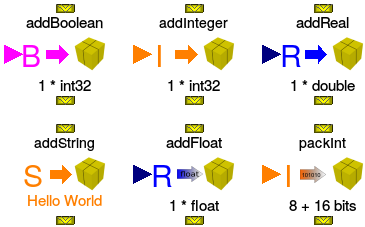
\includegraphics[width=0.6\columnwidth]{figures/SerialPackagerBlocks}
  \caption{\modelica{SerialPackager} blocks for adding variables to a package.}
  \label{fig:SerialPackagerBlocks}
\end{figure}

At the C side, a package is a C byte array in which C variables with
respectively indicated types are simply successively appended in a data-flow
prescribed order. For example, in Figure~\ref{fig:PackagingConcept} the
resulting byte array starts with three \clang{double} values ($3 \times 8$ bytes)
followed by one \clang{int32} value ($4$ bytes), resulting in a byte array of size 28.
For the sake of providing an illustrative example at the C language level
the following C code snippet constructs a structurally equal package named
\clang{data} (the example shall shed light on the concept, it does not
advocate a coding style using magic numbers for array offsets):
\begin{lstlisting}[language=C]
double v1[3] = {1.1, 2.2, 3.3};
int v2 = 4;
unsigned char* data = (unsigned char*) calloc(28, sizeof(unsigned char));
memcpy(&data[0], &v1[0], sizeof(v1));
memcpy(&data[24], &v2, sizeof(v2));
\end{lstlisting}
Figure~\ref{fig:SerialPackagerBlocks} shows the blocks for adding
variables to a package, symmetrically, blocks are available for retrieving variables from a
package. Using these blocks is deemed to be rather
intuitive with the notable exception of the \modelica{packInt} block. This
block allows to pack unsigned integer values at the bit level. The number of
bits used for encoding is set by a parameter \modelica{width}, therefore the maximum value
of the integer signal that can be encoded is $2^{\mathrm{width}} - 1$. A
parameter \modelica{bitOffset} allows to specify the bit at which the encoding starts
relative to the preceding block. Since MDD v1.3 most blocks support specifying
the byte ordering (big-endian or little-endian format).

It is simple to use the
\modelica{SerialPackager} blocks for deserializing data which has been serialized by it
(see Figure~\ref{fig:PackagingConcept}). In practice, however, communication
typically needs to be established with a remote station which is unrelated to
the Modelica model. As long as this remote station periodically sends or
receives structurally static, fixed sized packages it is usually quite
convenient to establish a communication using the MDD blocks. If the remote
station uses a more dynamic protocol it becomes more difficult. In some cases
using the \textsf{Function Layer} directly (instead of the \textsf{Block Layer})
can provide additional flexibility for coping with more dynamic protocols.
However, the main use-case for the \modelica{SerialPackager} concept is periodically
sent, structurally static data. This restrictions may be relieved in
future versions of MDD by providing additional ``Packagers'' that support more
flexible means of packaging data.

It turned out that the \modelica{SerialPackager} blocks were a major hurdle for
extending the number of Modelica tools which support MDD. They use a rather
intricate mechanism for propagating a ``package'' between connected blocks
which is discussed further in Section~\ref{sec:ModelicaStandardCompliance}.

\subsubsection{Hardware I/O}

Package \modelica{HardwareIO} (see
Figure~\ref{fig:MDDPackageBrowseScreenshot}) is intended for data acquisition
hardware like digital-analog converter (DAC), analog-digital converter (ADC) and
other interface hardware.

\begin{figure}[htb]
  \centering
  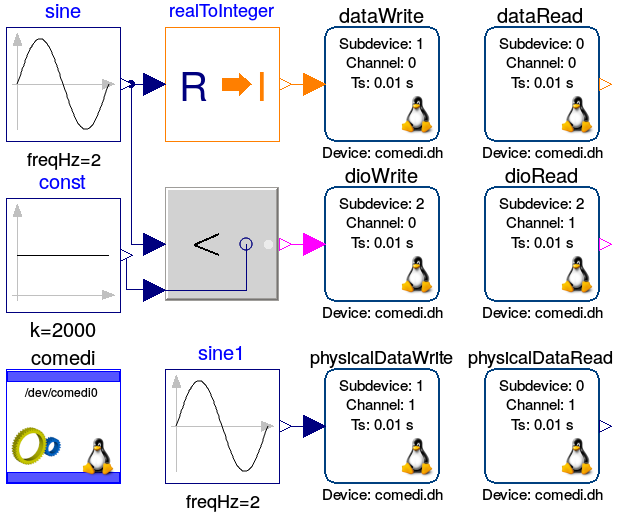
\includegraphics[width=0.9\columnwidth]{figures/MDDComedi}
  \caption{Accessing data acquisition hardware via the Linux
  control and measurement device interface ``Comedi''.}
  \label{fig:MDDComedi}
\end{figure}

\noindent
As of MDD v1.5.0 it contains only one sub-package which
provides support for the Linux control and measurement device interface
``Comedi''. The Comedi project develops open-source drivers, tools, and
libraries for data acquisition\footnote{Comedi project,
\url{http://www.comedi.org}}. The project provides a common interface for
accessing supported data acquisition hardware (see the website for supported
hardware). The MDD library implements an interface to the Comedi user-space
library.

Figure~\ref{fig:MDDComedi} shows an example model which uses the available
blocks. Configuration of the device is performed in the Modelica record named
\modelica{comedi}. The record contains an external object \modelica{dh} of type
\modelica{ComediConfig} which contains the Comedi device handle and is passed through
a parameter to the other blocks (\modelica{comedi.dh}). Using external
objects in records is not standard compliant to Modelica v3.3 revision 1
\citep{ModelicaAssociation2014} which is further discussed in
Section~\ref{sec:ModelicaStandardCompliance}.

Writing or reading raw integer values to DAC or from ADC channels is provided by
blocks \modelica{DataWrite} or \modelica{DataRead}, respectively. These blocks have
each a variant which works with physical values, instead of the raw integer
values  (\modelica{PhysicalDataWrite} and \modelica{PhysicalDataRead}).
Blocks \modelica{DIOWrite} and \modelica{DIORead} support digital input and
output (DIO) channels.

\subsubsection{Embedded Targets}
\label{sec:EmbeddedTargets}

MDD v1.5.0 introduced the new top-level package \modelica{EmbeddedTargets}. The
package is intended for platform-specific targets, such as microcontrollers,
that cannot so easily share code with other devices due to memory or hardware
limitations.
There exists first prototypical support for the
Atmel\footnote{Atmel, \url{http://www.atmel.com}} AVR family of
microcontrollers. A prototype application is described in
Section~\ref{sec:EmbeddedControl}.

\section{Modelica Standard Compliance}
\label{sec:ModelicaStandardCompliance}
\BTHI{TODO: Thomas, Bernhard}

Using a Modelica library-based approach for accessing hardware devices from a
simulation started as an experiment which relied on the Dymola tool and its
support for interfacing external C code.
% The result was the \emph{ExternalDevices} library, the historical predecessor of
% the MDD library (see Section~\ref{sec:Introduction}).
However, when trying to extend the number
of Modelica tools which support the MDD library, it became apparent that quite a
few constructs that were useful and appreciated by the initial authors of the
library were not supported by other tools and were partly problematic in respect
of compliance to the Modelica standard.

On one hand, this section reports on
important development efforts (starting with MDD v1.4.0) that have been spent on the
Modelica compliance of the library for better supporting SimulationX and
OpenModelica, and on the other hand it addresses open issues which may
be of interest for future improvements to the Modelica standard, or which
may require possibly non-backwards compatible revisions of the MDD library for
achieving full Modelica compliance.

\subsection{Modelica's External Function Interface}

Modelica's external function interface specification improved over the years,
which allowed to create more satisfying, standard-conform libraries with
external C code dependencies. For example, Modelica v3.2
introduced a standardized directory structure for searching for
external libraries \citep[p.\@~153]{ModelicaAssociation2010}:
\begin{tabbing}
pa\=ck\=ag\=e.mo {\small// contains the Modelica code}\\
\texttt{\textbf{Resources}}\\
\>\texttt{\textbf{Include}}\\
\>\>Ext1.h {\small// C-header file}\\
\>\texttt{\textbf{Library}}\\
\>\>\texttt{\textbf{win32}}\quad {\small// Windows 32 bit libraries}\\
\>\>\>ExtLib1.lib {\small// static link library for VisualStudio}\\
\>\>\>ExtLib2.lib {\small// statically linking the dynamic link library}\\
\>\>\>ExtLib2.dll {\small// dynamic link library (with manifest)}\\
\>\>\texttt{\textbf{win64}}\\
\>\>\>{\small// Windows 64 bit versions of above libraries}\\
\>\>\texttt{\textbf{linux32}}\quad {\small// Linux 32 bit libraries}\\
\>\>\>ExtLib1.a {\small// static link library}\\
\>\>\>ExtLib2.so {\small// shared library}\\
\>\>\texttt{\textbf{linux64}}\\
\>\>\>{\small// Linux 64 bit versions of above libraries}\\
\end{tabbing}
Having this standardized directory structure (which was missing in Modelica
v3.1) facilitated creating cross-platform libraries with external C library
dependencies. For example, the Modelica code snippet below declares a
dependency to the header file \modelica{ExtFunc1.h} and the libraries
\modelica{ExtLib1} and \modelica{ExtLib2}:
\begin{lstlisting}[language=modelica]
function getFoo
  input Real u;
  output Real y;
  external "C" y = Ext1_getFoo(u)
    annotation(Include = "#include \"Ext1.h\"",
    Library = {"ExtLib1", "ExtLib2"});
  annotation(__ModelicaAssociation_Impure=true);
end getFoo;
\end{lstlisting}
A Modelica tool will map these information to compiler- and linker-dependent
directives and thereby select the libraries which fit best for the respective
platform.

The example features an additional annotation which declares the function
as ``impure''. The intended meaning is that a tool may not expect that the
function returns the same output for the same input, which is the typical case
for MDD functions which read values from external devices. Indeed, Modelica v3.3 introduced the dedicated keyword
``impure'' to cater for such cases. However, since not all tools support this
keyword, yet, the MDD library uses the featured annotation which is understood
by all the tools known to support the MDD library.

\subsection{The Serial Packager}

The \modelica{SerialPackager} blocks are core elements of the block-based
communication support provided by the MDD library (see
Section~\ref{sec:Communication}). They use a rather intricate mechanism for
propagating a “package” between connected blocks which is discussed in this
section.

\subsubsection{Connector Definition}

The definition of the \modelica{SerialPackager} input connector is given below.
\begin{lstlisting}[language=modelica]
connector PackageIn "Packager input connector"
  input SerialPackager pkg;
  input Boolean trigger;
  input Real dummy;
  output Boolean backwardTrigger;
  output Integer userPkgBitSize;
  output Integer autoPkgBitSize;
end PackageIn;
\end{lstlisting}
The definition of the output connector is similar, but with reversed input and
output causalities. Most notably connector \modelica{PackageIn} contains an
element \modelica{pkg} which is an external object of type \modelica{SerialPackager}.
This external object is passed between connected blocks (see
Figure~\ref{fig:PackagingConcept}). Within an ``add'' or ``get'' block the
passed in external object is used as an argument to external functions which
first add or retrieve data from the package and when pass it on to the next block.

\subsubsection{Basic Concept}

The
following \emph{simplified} Modelica code snippet illustrates the basic idea for
adding the value of an input variable \modelica{u} to a package:
\begin{lstlisting}[language=modelica]
block AddValue
  PackageIn pkgIn "Input connector";
  PackageOut pkgOut "Output connector";
  IntegerInput u "Integer input connector";
equation
  when initial() then
    pkgIn.autoPkgBitSize = pkgOut.autoPkgBitSize + 32;
  end when;
  when pkgIn.trigger then
    pkgOut.dummy = addValue(pkgOut.pkg, u, pkgIn.dummy);
  end when;
  pkgOut.pkg = pkgIn.pkg;
  pkgOut.trigger = pkgIn.trigger;
  pkgOut.backwardTrigger = pkgIn.backwardTrigger;
  pkgOut.userPkgBitSize = pkgIn.userPkgBitSize;
end AddValue;
\end{lstlisting}
The instantaneous equation \modelica{addInteger} is activated by the event
\modelica{trigger} which is propagated through the connected packager blocks.
The \modelica{dummy} variables are used to establish data-flow dependencies
which ensure that (external) ``\modelica{addValue}'' functions in connected
blocks are called in the correct order. The \modelica{backwardTrigger} event
allows to propagate a triggering event in the inverse connector direction.
Its supporting logic is omitted here for brevity. Variable
\modelica{userPkgBitSize} allows to propagate a user defined package size which
can be set at a communication device block, \textit{e.g.}, it is possible for a
user to specify that the size of the external C ``\modelica{data}'' buffer (see
Section~\ref{sec:Communication}) of a package should be eight bytes. However,
the default setting is that the necessary package size is deduced automatically
with the help of the \modelica{autoPkgBitSize} variable. The mechanism is
described further below.

\subsubsection{External Object Aliasing}
\label{sec:External Object Aliasing}

A problem with the \modelica{AddValue} block is that the \modelica{pkg}
objects within the connectors are not explicitly created by calling an external object constructor
function as required in the Modelica v3.3 \cite[p.\@~165]{ModelicaAssociation2014}.
Instead, they rely on aliasing through equations and connection equations to
access an external object which has been created at another place. In
Figure~\ref{fig:PackagingConcept} the \modelica{pkg} object for the ``add''
blocks is created in the  ``Packager'' block at the top of the figure, while the
\modelica{pkg} object for the ``get'' blocks is created in the device block for reading from
shared memory (or UDP, respectively). While the concept of external object
aliases does not exist in Modelica v3.3, equating two external
objects may be interpreted as an assignment to an external object,
which is forbidden. The authors hope that future versions of
the Modelica standard will consider use-cases such as the one described above
and allow them explicitly.

\subsubsection{Automatic Buffer Size}

The actual creation of the \modelica{SerialPackager} object is performed in
the ``Packager'' block, or, respectively, in the reading device block (see
above). The following \emph{simplified} code illustrates the basic concept.
\begin{lstlisting}[language=modelica]
block Packager
  PackageOut pkgOut(
    pkg = SerialPackager(bufferSize),
    dummy(start=0, fixed=true));
  Integer bufferSize;
equation
  when initial() then
    bufferSize =
      if pkgOut.userPkgBitSize > 0 then
      pkgOut.userPkgBitSize else
      pkgOut.autoPkgBitSize;
  end when;
end Packager;
\end{lstlisting}
The difficulty here is that the \modelica{bufferSize} which is needed as an
argument for the external object constructor
\modelica{SerialPackager(bufferSize)} needs to be computed by solving the
initial system of equations. This is not supported by all Modelica tools and its
Modelica compliance was discussed at the Modelica Issue Tracker with a majority
opting to clarify the specification in order to forbid it\footnote{Modelica Issue Tracker,
\url{https://trac.modelica.org/Modelica/ticket/1907}}, but on the other hand
also proposals how the Modelica standard could be extended to allow
it\footnote{Modelica Issue Tracker,
\url{https://trac.modelica.org/Modelica/ticket/2037}}.

In the initial version of the MDD library the external object was actually
created within the when clause, like,
\begin{lstlisting}[language=modelica]
when initial() then
  pkgOut.pkg = SerialPackager(bufferSize);
end when;
\end{lstlisting}
which was clearly illegal in Modelica v3.3. As part of improving the Modelica
compliance of the library the creation of the object was moved into the
component declaration.

\subsection{External Objects in Records}

The SocketCAN and the Comedi blocks use a Modelica \modelica{record} as means
for specifying general settings for a hardware device. The idea is that the
settings are specified once when creating an instance of the record and
this instance is passed as parameter to blocks which use this device. For
example, the Comedi configuration record (stripped from some elements for brevity) is defined
as
\begin{lstlisting}[language=modelica]
record ComediConfig
  parameter String deviceName =
    "/dev/comedi0" "Name of Comedi device";
  final parameter Comedi dh =
    Comedi(deviceName) "Handle to comedi device";
end record;
\end{lstlisting}
where \modelica{dh} is an external object. It is convenient to collect
configuration information in a record, since this allows to pass a complete set
of related configuration settings at once. The problem here is that passing an
external object as part of a record can be interpreted as the record returning
the object and assigning it to another external object (which is forbidden in
Modelica v3.3). However, similarly to the external object aliasing described in
Section~\ref{sec:External Object Aliasing} it seems highly desirable to consider
use-cases as described above in some way,  in future versions of the Modelica
standard.


% \subsection{Enhancements}
% \subsection{Pitfalls and Open Issues}
% Aide-mémoire:
% \begin{itemize}
%   \item Serialpackager
%   \item Automatic buffer size
%   \item External objects in equation
%   \item Construction of external objects in record
%   \item Linking to platform-dependent system libraries
%   \item Missing fixed attribute for String
%   \item Support of several include directories
% \end{itemize}

\section{Applications}
\label{sec:Applications}

This section describes several applications which were implemented with the
help of the MDD library.

\subsection{Arduino}
\BTHI{TODO: Volker}
\TBEU{TODO: Improve double wording ''With the help of''}

The Arduino\footnote{Arduino, \url{https://www.Arduino.cc}} is an open-source electronics platform which makes it very easy to read sensors, process the data and send it to another device via a serial connection.
With the help of the MDD serial port implementation, the Arduino can be utilized to make sensor data available in a real-time Modelica model, as depicted in Figure~\ref{fig:arduino} \footnote{Autodesk screen shots reprinted courtesy of Autodesk, Inc.}.
With the help of potentiometers or other deflection sensors, customized control devices can be built.

As an exemplary application, self-built pedals for a driving simulator can be equipped with a sensor in order to measure the displacement. The pedal itself is a steel sheet, mounted on a revolute joint and a shock spring.
The measured deflection is transferred via a serial connection to a \modelica{Blocks.Communication.SerialPortReceive} in order to drive a virtual vehicle.
Therefore, expensive or unavailable input devices can be substituted by custom constructions.
\begin{figure}[htb]
  \centering
  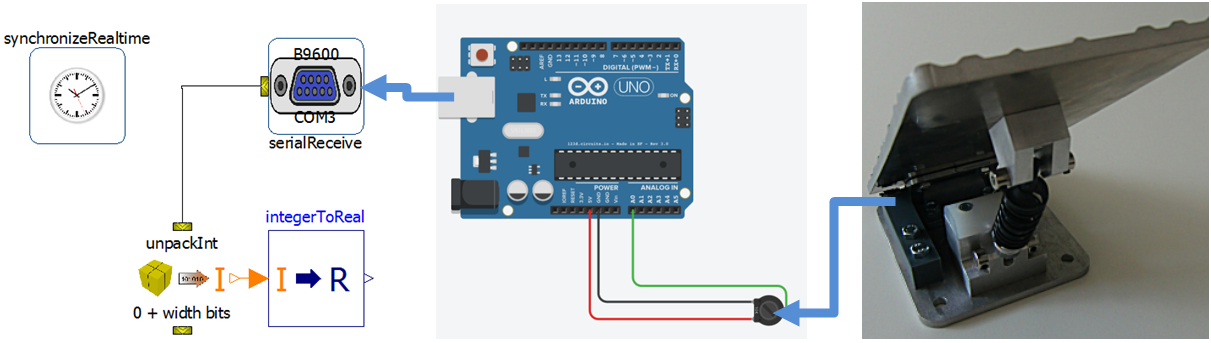
\includegraphics[width=0.9\columnwidth]{figures/arduino}
  \caption{Setup to read potentiometer deflection during real-time simulation with MDD serial port model.}
  \label{fig:arduino}
\end{figure}

\noindent
By using a Bluetooth module with Serial Port Profile (SPP) a wireless connection between Arduino is handled in the same way as a serial port over USB connection.
No further modifications are necessary to implement a wireless control device.

\subsection{Embedded Control}
\label{sec:EmbeddedControl}

% The MDD library has been extended to support simulation of Modelica models
% running on microcontrollers. Since microcontrollers have very limited
% hardware, no threading support, limited memory allocation, \textit{etc.}, the
% general-purpose external functions in MDD cannot be used.

The \modelica{EmbeddedTargets} package (see Section~\ref{sec:EmbeddedTargets}) contains
blocks and functions to directly control I/O or clocks in the AVR ATmega microcontroller family\footnote{As of MDD
v1.5.0, only ATmega16 and ATmega328P (=Arduino Uno) are supported.
The code can easily be extended, but requires checking the data sheets in order
to write to the correct bits.}.
The advantage of including this code into the MDD library is that it makes it
simple to write a model for a microcontroller that works the same way
in any Modelica tool since all the OS support, real-time code, etc is
abstracted away.
Provided that the Modelica tool produces minimal C-code (uses minimal features
outside of standard C: for example, no linear solver included if the system has no linear systems,
no OS or I/O functions, no threading models, etc),
and the model itself does not use C-code that the embedded target cannot support
(such as file I/O), the code generator would work on pretty much any embedded
target supporting C.

The Modelica code itself tries to avoid the Integer constants from the
data sheets.
Instead, enumerations such as \modelica{prescaler}=1/128 or \modelica{clock}=2B are
passed from Modelica and the C code for the AVR target depends on
function inlining in order to remove dead code.
For example, the constructor for the clock takes an enumeration which
specifies the clock which should be manipulated and after function inlining, the
C code for other clocks is removed.
The blocks in the MDD library try to take user-friendly constants
such as \modelica{frequency}=$100\,\mathrm{Hz}$ or \modelica{period}=$0.1\,\mathrm{s}$ for real-time synchronization; the
Modelica code then has logic to find good clock prescalers to create a
matching frequency.
The code does not use parameters since they cannot be guaranteed to be
evaluated in Modelica, and the C-code depends on the C-compiler (AVR GCC)
being able to inline and eliminate dead code from C-code such as the constructor.
An example of this is the timer external object in the microcontroller which becomes one or two bitset
instructions when the function is called with a constant input:
\begin{lstlisting}[language=Modelica]
function constructor "Initialize timer"
  input Types.TimerSelect timerSelect;
  input Types.TimerPrescaler clockSelect;
  input Boolean clearTimerOnMatch;
  output Timer timer;
  external "C" timer = MDD_avr_timer_init(timerSelect, clockSelect, clearTimerOnMatch)
    annotation(Include="#include \"MDDAVRTimer.h\"");
end constructor;
\end{lstlisting}
\begin{lstlisting}[language=C]
static inline void* MDD_avr_timer_init(int timerSelect, int clockSelect, int clearTimerOnMatch)
{
  static const uint8_t
    clockSelectTable0[7] = {...},
    clockSelectTable1[7] = {...},
    clockSelectTable2[7] = {...};
  switch (timerSelect) {
#if defined(TCCR0)
  case 1: /* Timer 0 */
    TCCR0 |= ...;
    break;
#elif defined(TCCR0B)
  case 1: /* Timer 0 */
    TCCR0B |= clockSelectTable0[clockSelect-1];
    TCCR0A |= ...;
    break;
#endif
  case 2: /* Timer 1 */
    ...
  case 3: /* Timer 2 */
    ...
  default:
    exit(1);
  }
  return (void*)timerSelect;
}
\end{lstlisting}
One of the AVR examples included in MDD is the single board heating system (SBHS\footnote{SBHS, \url{http://sbhs.fossee.in/}}), shown in Figure~\ref{fig:sbhs}.
\begin{figure}
  \centering
  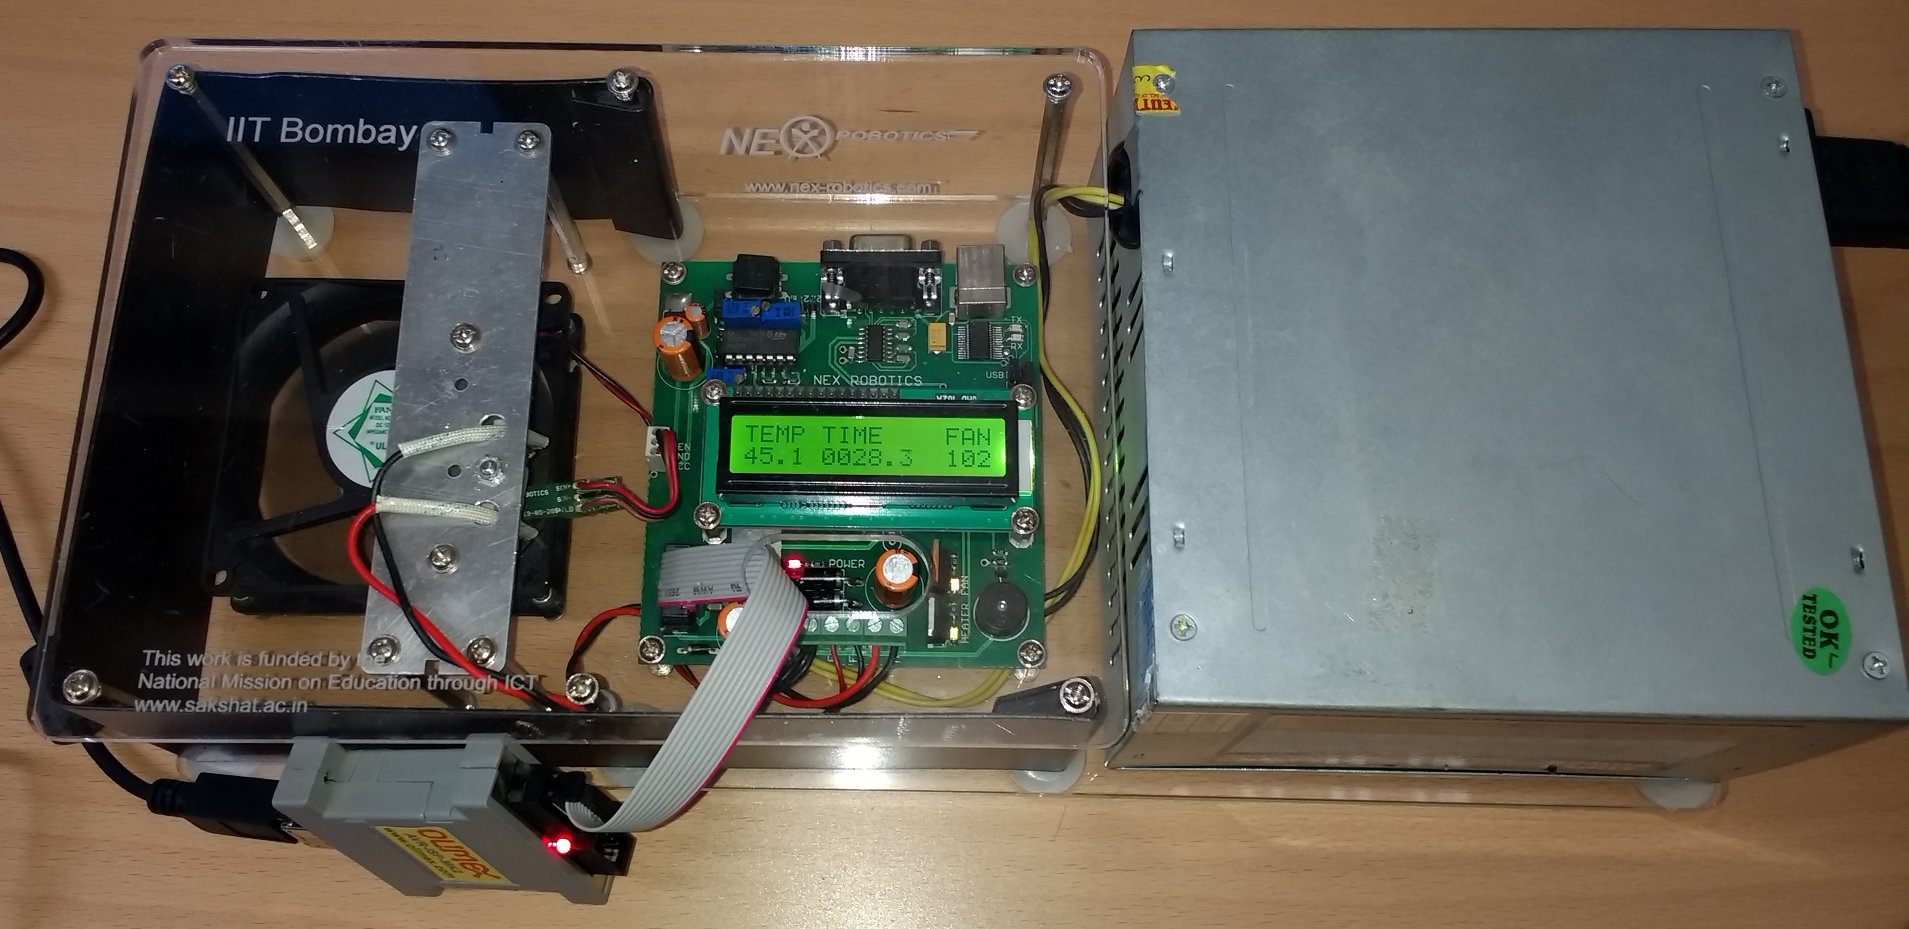
\includegraphics[width=0.9\columnwidth]{figures/SBHS.jpg}
  \caption{The single board heater system running a real-time control algorithm using firmware based on MDD code. There is a programmer attached to the board to upload new firmwares, but the code runs without any computer connected to the SBHS.}
  \label{fig:sbhs}
\end{figure}
The SBHS consists of a heater assembly, fan, temperature sensor, AVR ATmega16 microcontroller and associated circuitry.
It was developed by IIT Bombay and is used for teaching and learning control systems \cite{Arora2010}.
The MDD SBHS example uses a model of the board (Figure~\ref{fig:sbhsboard})
\begin{figure}
  \centering
  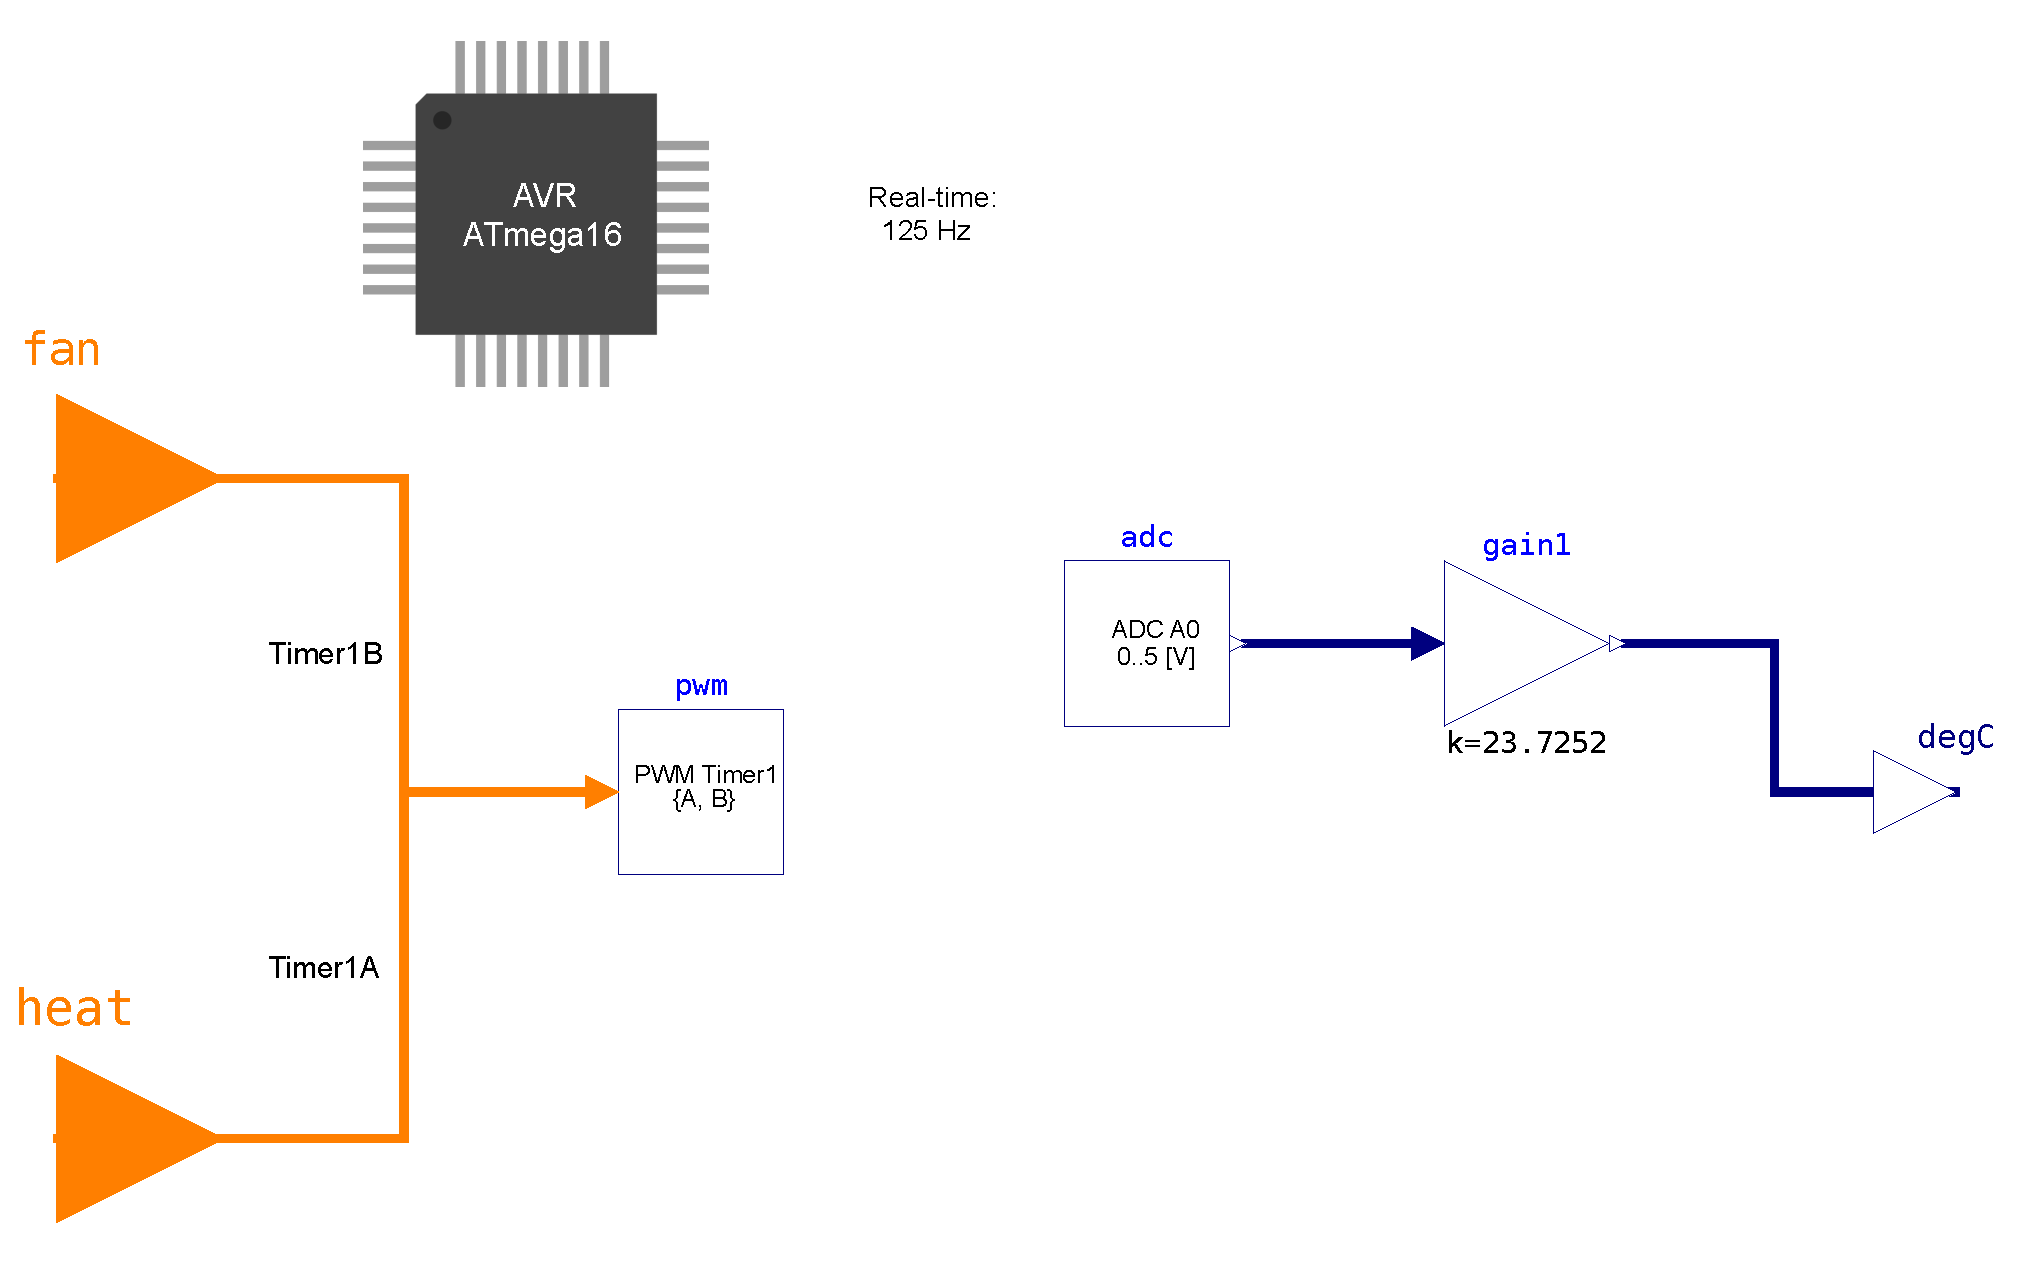
\includegraphics[width=0.9\columnwidth]{figures/SBHSBoard.pdf}
  \caption{The MDD model of the single board heater system exposes the pulse-width modulation (PWM) block to control the heater and fan, and uses the analog-to-digital converter (ADC) block to read the temperature. Note that the SBHS board uses hardware components to create a linear mapping from voltage to temperature where $0\,\mathrm{V}$ maps to $0\,$℃.}
  \label{fig:sbhsboard}
\end{figure}
\begin{figure}
  \centering
  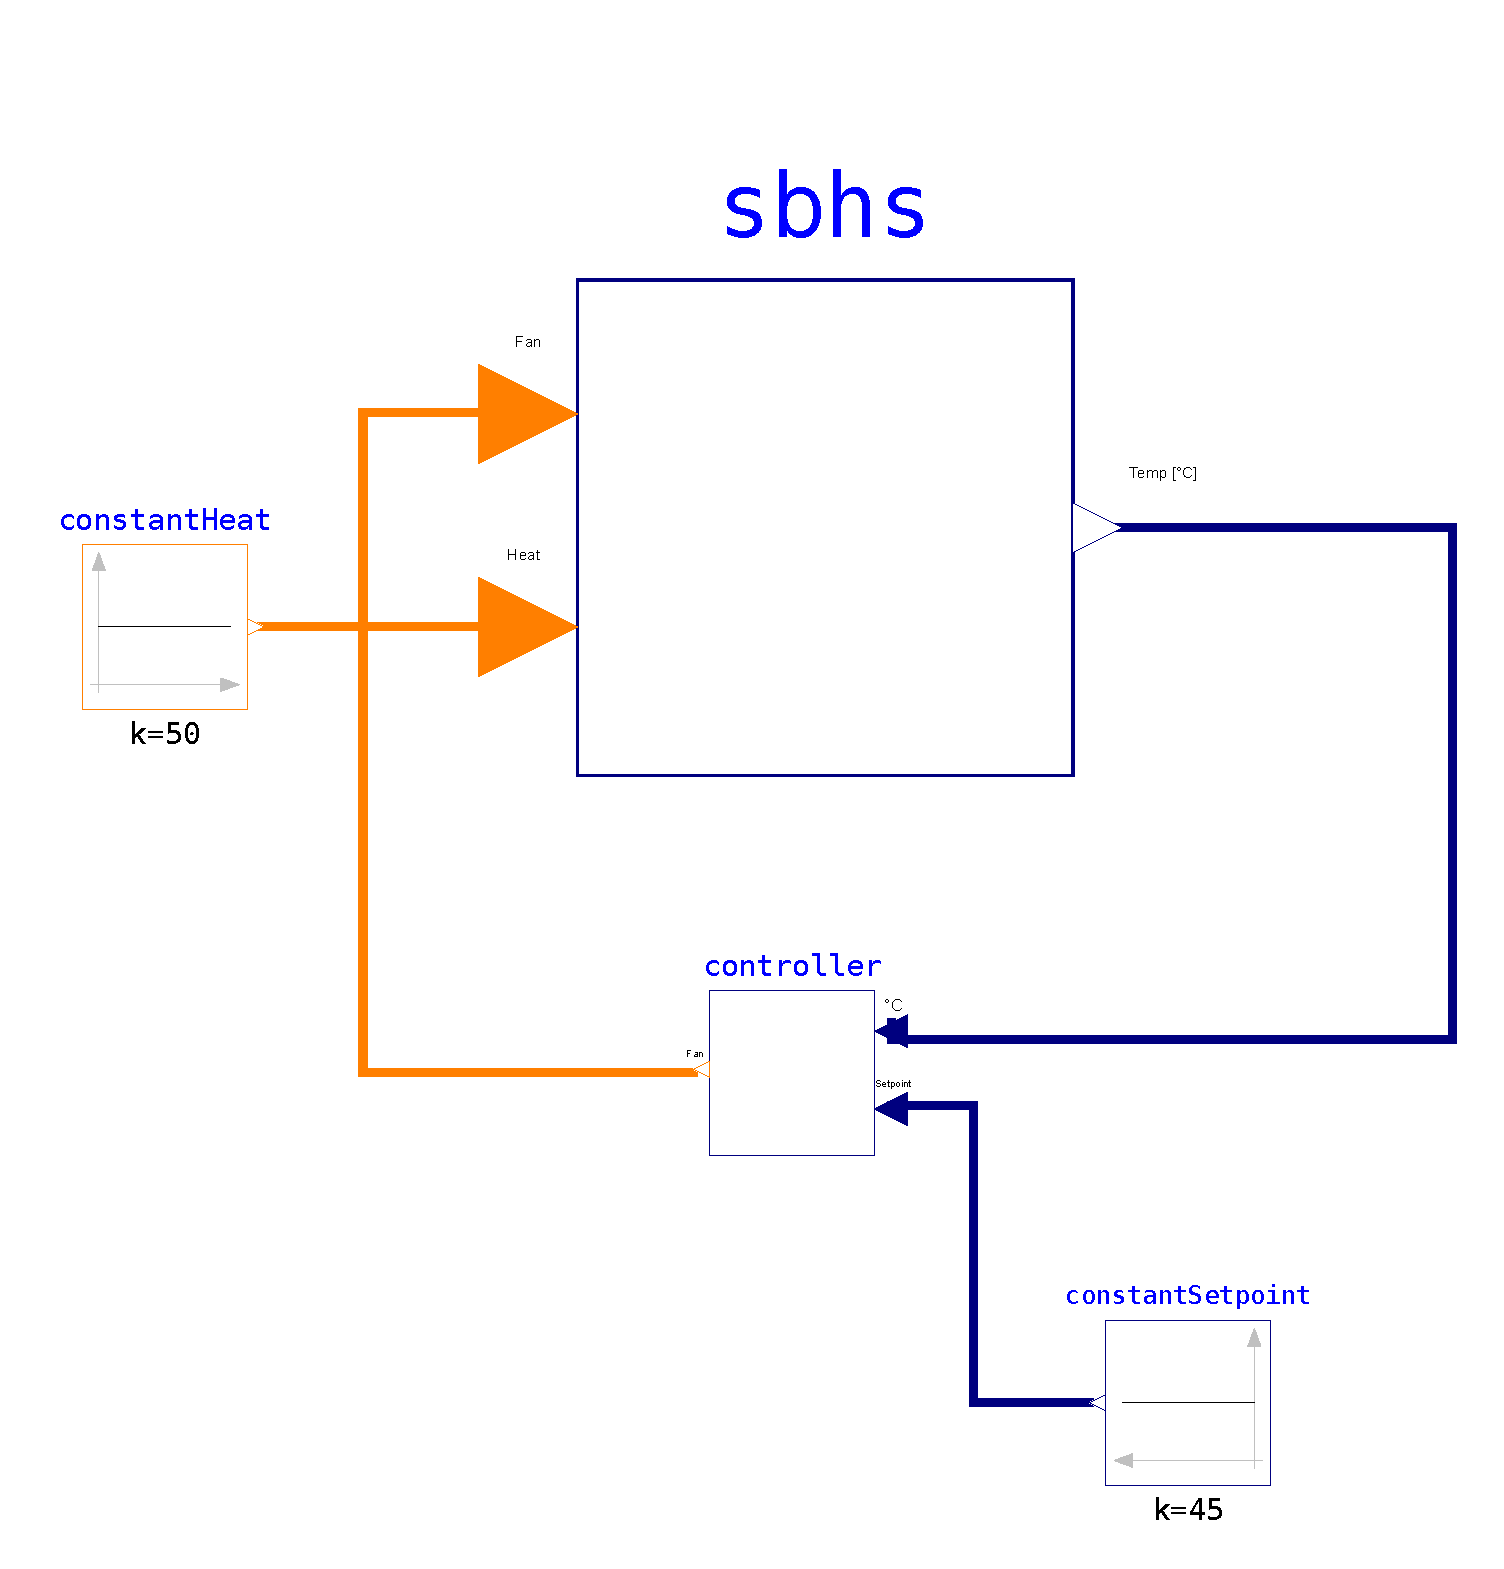
\includegraphics[width=0.5\columnwidth]{figures/SBHSBoardWithController.pdf}
  \caption{The MDD example model of the single board heater system running at $125\,\mathrm{Hz}$ together with a real-time PID controller trying to control the fan such that the temperature is at the setpoint of $45\,$℃ while the heat source is fed by a constant voltage.}
  \label{fig:sbhswithcontroller}
\end{figure}
and a simple controller which it combines into the real-time controller of the board (Figure~\ref{fig:sbhswithcontroller}).

% The \modelica{EmbeddedTargets} models do not support simulating the microcontroller
% on a desktop platform. This would be an interesting, but time-consuming
% extension to the work.

\subsection{DLR Demonstrators}
\BTHI{Tobias}

At the DLR Institute of System Dynamics and Control, several simulator systems
utilize the MDD library for inter-system
communication and querying of input devices.

\begin{figure}[htb]
  \centering
  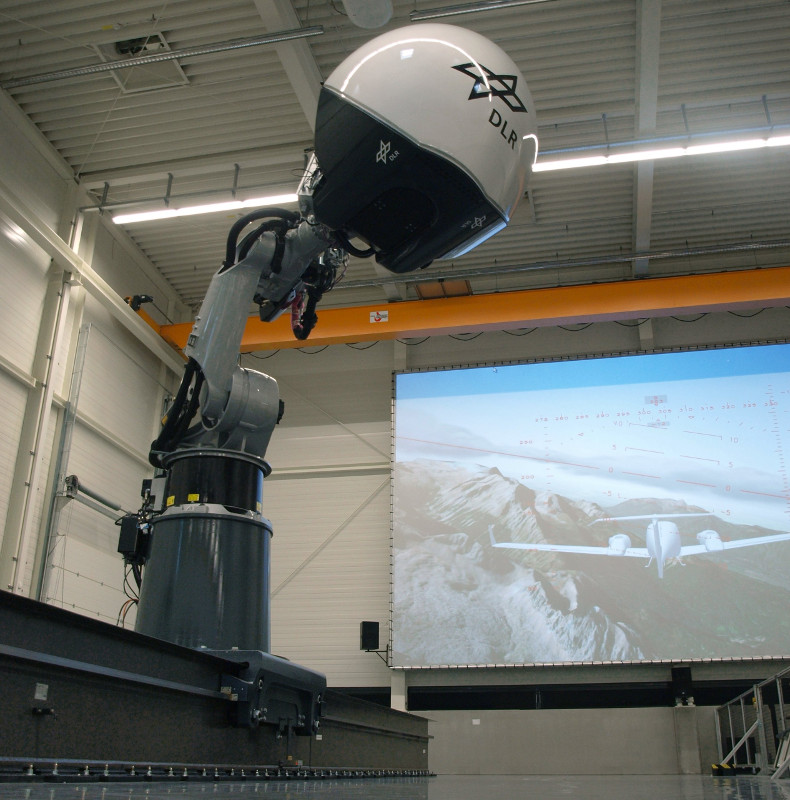
\includegraphics[width=0.9\columnwidth]{figures/DLRRoboticMotionSimulator}
  \caption{The DLR Robotic Motion Simulator.}
  \label{fig:DLRRoboticMotionSimulator}
\end{figure}

\noindent
The DLR Robotic Motion Simulator \citep{bellmann2011dlr} is a 7 axis driving and
flight simulator based on an industrial robot arm (see
Figure~\ref{fig:DLRRoboticMotionSimulator}). The main use of this motion
simulator is the evaluation of input devices such as side-sticks, steering
wheels, pedals, etc., as well as the test and validation of control algorithms
in terms of stability and real-time capability. The control architecture of the
simulator uses blocks from the MDD library in several ways:
\begin{itemize}
  \item Input devices such as force-feedback steering wheels are connected via CAN bus
and integrated in the software framework via the CAN blocks, the same
applies for a force-feedback side-stick.
  \item Other, consumer based input devices such as pedals or Airbus styled flight
controls are connected via the \modelica{JoystickInput} block.
  \item The control architecture for the robot consists of two Modelica simulations on
two different computers: First, the real-time path-planning running on a
real-time Linux system controlling the movements of the robot, and second, the
control panel running on a standard Windows system. The control panel is used to
change parameters such as washout filter modes (the washout filter maps the
movement of road vehicles / airplanes to the workspace of the simulator) and
gives an overview on the actual robot's position and telemetry. All real-time critical
communication (\textit{e.g.}, the simulated road vehicle / airplane forces and
angular velocities inputs for the real-time path-planning, or the control panel
I/O) are communicated via the UDP blocks and the serial
packaging system.
\end{itemize}

\begin{figure}[htb]
  \centering 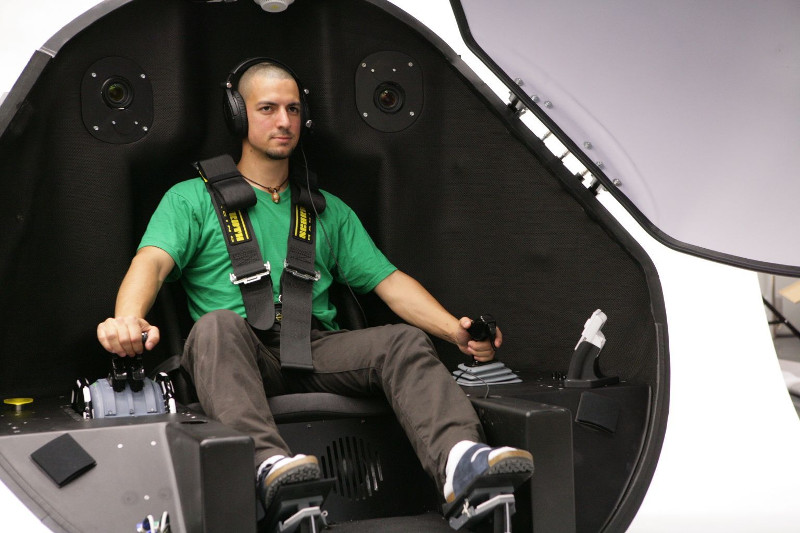
\includegraphics[width=0.9\columnwidth]{figures/DLRSimulatorCabin}
  \caption{View into the simulator cabin of the DLR motion simulator. The
  instrumentation package is replaceable, so that the simulator cabin can be
  easily adapted for different simulation types, \textit{e.g.}, for driving or
  flight simulation.}
  \label{fig:DLRSimulatorCabin}
\end{figure}

\noindent
Figure~\ref{fig:DLRSimulatorCabin} shows the inside of the simulator cabin.
The instrumentation package can be adapted
for different simulation types or for testing different input concepts.
An on-board computer is used to query input devices, to display information on
control screens, and to project the pilot's outside view visualization on the
embracing concave dome shell. These
tasks are performed using Modelica models, where the
\modelica{SynchronizeRealtime} block is used for real-time
synchronization. Also, communication with the other simulation components is
performed partly via the UDP blocks.

\begin{figure}[htb]
  \centering
  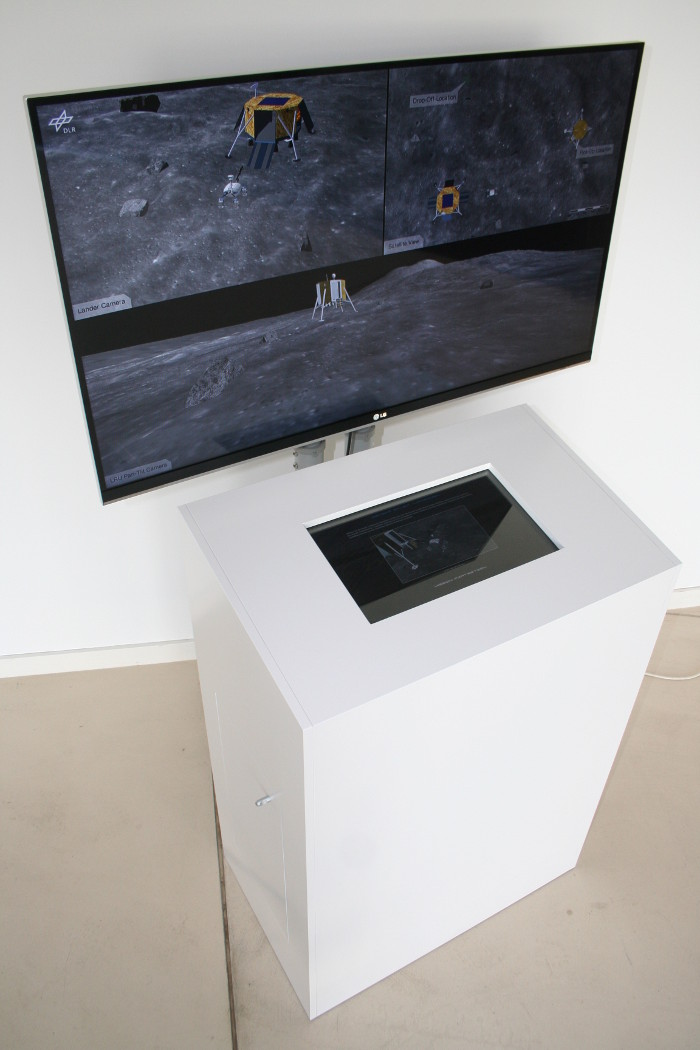
\includegraphics[width=0.5\columnwidth]{figures/DLRROBEX}
  \caption{DLR ROBEX technology demonstrator.}
  \label{fig:DLRROBEX}
\end{figure}
\TBEU{Tobias: Do you have any citable references for the application or exhibition?}
Figure~\ref{fig:DLRROBEX} shows the ROBEX demonstrator which was developed as a technology demonstrator
for a science exhibition.
This demonstrator allows the user to command a rover
on a scientific lunar mission. The mission's goal is to pick up a sensor package from a nearby
lander and to place it on a marked position on the lunar surface. The user
controls the rover via an Android App which is running on a tablet computer in front of
the simulator screen.
\TBEU{Bernhard: Add link to Android in footnote?}On the screen, the visualization of the rover is displayed.
The underlying Modelica simulation performs the multi-body simulation of the
rover and utilizes the \emph{DLR Visualization} library to display the rover and the
scenery.
\TBEU{Tobias: Which MDD blocks exactly? I assume UDP Receiver. Is the Android App open-source and can be added as link in a footnote?}It uses MDD blocks to communicate with the tablet computer and the
\modelica{SynchronizeRealtime} block to adjust the simulation speed.

In very similar ways, the library is also used in several other simulator and
demonstrator systems, \textit{e.g.}, a drilling rig training simulator, several
desktop flight simulators, or a rover software-in-the-loop development
environment.

\section{Outlook}
\BTHI{TODO: Bernhard, Thomas, Volker}
% Generalization of the SerialPackager by other serializers like XDR or LCM (based on XDR) might be a realistic goal

The \emph{Modelica\_DeviceDrivers} library is a tried and tested library which
can support a wide range of application scenarios. During its development
valuable experience on interfacing Modelica with external C code has been
gained. Thus, the source code can also serve as an example for anybody who is
interested in applications which require a more complex integration of Modelica
code with external C code.

Considerable development efforts have been spent on improving the Modelica
compliance of the library. Still, there are open issues and one may also see the
library as a testbed which stresses Modelica's external function interface
to the limit. On one one hand, experiences gained thereby can provide inputs for
further enhancements to the Modelica standard specification, on the other hand,
further efforts in the library development can improve the level of standard compliance.
However, since backwards compatibility is a strong objective in the library
development, non-backwards compatible changes for the sake of better
standard compliance will not be introduced lightly.

Naturally, there is a large pool of conceivable feature extensions to the
library, due to the myriad number of available external devices and
communication protocols. A frequent request is to extend the communication
abilities beyond the capabilities of the available \modelica{SerialPackager}.
There exists a huge choice of data serialization formats which could be utilized for this
purpose. Particularly, with regard to Internet of Things (IoT) technology
becoming more important, improving communication capabilities is a worthy goal.
Similarly, supporting embedded systems is very attractive in that perspective
and first prototypical work in that direction has been briefly outlined in this
paper.

\section*{Acknowledgements}

Support of Linköping University by VINNOVA in the ITEA3 OPENCPS project and
in the RTISIM project (Strategic Indo-Swedish Cooperative Innovation
Programme) is highly appreciated. The Open Source Modelica Consortium supports
the OpenModelica project.

Finally, we would like to thank everybody who has contributed to the library,
either by providing feedback and suggestions, or by direct contributions to
the implementation of the library, particularly, Miguel Neves, Dominik Sommer,
Rangarajan Varadan, and Dietmar Winkler.

%%% choose one of the following: %%%
%% References using bibtex (default)
\bibliography{modelica2017_Modelica_DeviceDrivers}

%% References using biber and biblatex
%\printbibliography

\end{document}
